\documentclass{article}

% if you need to pass options to natbib, use, e.g.:
% \PassOptionsToPackage{numbers, compress}{natbib}
% before loading nips_2016
%
% to avoid loading the natbib package, add option nonatbib:
\usepackage[nonatbib]{nips_2017}
\usepackage{nips_2017}

% to compile a camera-ready version, add the [final] option, e.g.:
% \usepackage[final]{nips_2016}

\usepackage[utf8]{inputenc} % allow utf-8 input
\usepackage[T1]{fontenc}    % use 8-bit T1 fonts
\usepackage{hyperref}       % hyperlinks
\usepackage{url}            % simple URL typesetting
\usepackage{booktabs}       % professional-quality tables
\usepackage{amsfonts}       % blackboard math symbols
\usepackage{nicefrac}       % compact symbols for 1/2, etc.
\usepackage{microtype}      % microtypography
\usepackage{graphicx}

\usepackage[style=apa,backend=biber]{biblatex}
\addbibresource{NIPS2017.bib}
\DeclareLanguageMapping{english}{american-apa}

\title{Enhancing learning performance and motivation by combining novelty seeking and hierarchical reinforcement learning}

\author{
  Maria K.~Eckstein \\
  Department of Psychology \\
  UC Berkeley \\
  Berkeley, CA 94720 \\
  \texttt{maria.eckstein@berkeley.edu} \\  
  \And
  Tom Griffiths \\
  UC Berkeley \\
  Address \\
  \texttt{tom_griffiths@berkeley.edu} \\
}

\begin{document}

\maketitle

\begin{abstract}
  We propose a novel task paradigm, which aims to differentiate reward-learning from novelty-learning, and thereby explains how structured, goal-directed behavior can arise in complex environment that are sparse in rewards. 
\end{abstract}

\section{Introduction}

It is desirable for a complex cognitive system, like a human, to understand its environment in a way that allows predictions about future states and events. This notion has been formalized in reinforcement learning theory (\cite{sutton_reinforcement_2017}), among others. Here, the agent tries to learn for each state (or feature of states, or abstract representation of states) how much "reward" to expect in the near future, given the agent's own action policy. Solving this prediction problem---knowing how much reward to expect at each state and from each action---interacts closely with the control problem---selecting actions as to maximize obtained reward. 

The balance between prediction and control, between acquiring a representation that allows for accurate predictions on one hand and the selection of reward-maximizing action on the other, has been phrased as a tension between exploration (prediction) and exploitation (control). And indeed, a cognitive system needs to explore its environment in order to learn a good representation, which in turn enables accurate predictions. But by definition, exploration reduces the number of exploitative, i.e., reward-maximizing actions, which implies that the two motives compete against each other for action selection and that exploration always comes at the cost of reducing pay-off and decreasing the quality of selected actions.

Challenging this view, recent research has shown that agents can acquire goal-directed behavior in the total absence of reward, i.e., in a purely exploratory setting (\cite{machado_learning_2016, singh_intrinsically_2004, tessler_deep_2016}). This shows that meaningful behavior is not tied to reward and exploitation as closely as is often assumed. One study (\cite{singh_intrinsically_2004}) achieved these surprising results by letting agents seek novelty instead of reward. The focus on novelty has been inspired by the structure of the mammalian brain; specifically, the brain's dopaminergic learning system responds similarly to novelty as to reward (\cite{wittmann_striatal_2008}). In addition, agents were provided with the ability to create "options", hierarchical action sequences, upon the encounter of novel events (\cite{sutton_between_1999}). In this setting, the novelty of easy-to-reach states decreased rapidly, forcing the agents to create more and more complex options in order to discover novel, but more remote events. This combination led to meaningful and structured behavior. 

A current theme in hierarchical reinforcement learning is the option-discovery problem (\cite{botvinick_model-based_2014}). Oftentimes, sub-goals are provided to the agent and the agent then only has to learn the policies to achieve these sub-goals. Once the policies are learned, the agent can select among these just like among basic actions, with considerable improvements in learning. But this depends crucially on the quality of the provided sub-goals. Much attention is therefore geared toward automatizing option discovery, i.e., creating agents that learn meaningful options on their own. Using novelty as a trigger for option creation, as suggested by the approaches mentioned above, might be one potential solution to this problem. 

In the current experiment, we tried to understand the emergence of complex, high-level, abstract thought from this perspective. We propose that abstract understanding is implemented through hierarchical structure (\cite{botvinick_model-based_2014}), and that meaningful hierarchical structure can be created by agents that employ novelty as a learning signal. In order to understand how complex, high-level, abstract cognition arises, we therefore aimed at studying the interaction between goal (reward versus novelty) and structure (flat versus hierarchical).

To this aim, we explored a spectrum of agents between "Sisyphus", a flat, reward-seeking agent on one hand, and "Socrates", a hierarchical, novelty-seeking agent on the other. The agents were exposed to a task with a complex underlying structure, but a simple quantitative goal. We hypothesized that the flat, reward-seeking Sisyphus agent would not learn meaningful behavior in this task, and instead bluntly repeat arbitrary actions. In addition, Sisyphus would continue to experience large negative reward prediction errors, equal to or greater in size that any positive prediction errors. We hypothesized that the hierarchical, novelty-seeking Socrates agent, on the other hand, would experience many positive prediction errors and show rapid learning of hierarchical options. Equipped with these, Socrates would be able to strategically explore the state space in order to discover more novel events, such that his overall reward prediction error balance would always be positive. 


\section{Methods}

\subsection{Environment / Task}

We created a task with both a concrete quantifiable goal, which invited the use of rewards and exploitation, and a complex, hard-to-predict structure, which invited the use of novelty and exploration. The task consisted of an array of turned-off lights, with the goal of lighting them all up. The agent was equipped with the two actions turn-on and turn-off, with the condition that only currently-off lights could be turned on and only currently-on lights could be turned off.

Unbeknownst to the agent, these basic or "0-level" lights were organized in groups of $n_{tuple}$ lights, e.g., groups of three in Figure \ref{TaskFigure}, and followed the subsequent rules. When the last light of a group was turned on, such that all lights of a group were lit-up at the same time, the environment responded with a novel event (such as a light of a different color), and also turned all lights of the group off again. We refer to the novel event as a first-level light. First-level lights were also organized into groups of $n_{tuple}$ lights. First-level lights produced a second-level light when turned-on at the same time and then turned off again. This same structure continued from one level to the next, making lights of higher levels increasingly "costly" to switch on. The number of levels was determined by the number of lights at the base level and by the number of lights per group. Higher-level lights could not be turned off directly; they only turned off when all lights in the same group were turned on, such that the whole group switched off.

Once a higher-level light was on, the corresponding lower-level lights would not extinguish any more if switched on at the same time. Therefore, the only way to turn on all the lights in the task was to first switch on the one highest-level light, than the $n_{tuple}$ lights of the level below, the $n_{tuple} ^ 2$ lights below this, and so on, until finally the all level-0 lights could be switched on. Switching on each higher-level light thereby required switching on several level-0 lights, some of them multiple times. Figure \ref{TaskFigure} shows an example illustration of the task.

\begin{figure}[h]
  \centering
  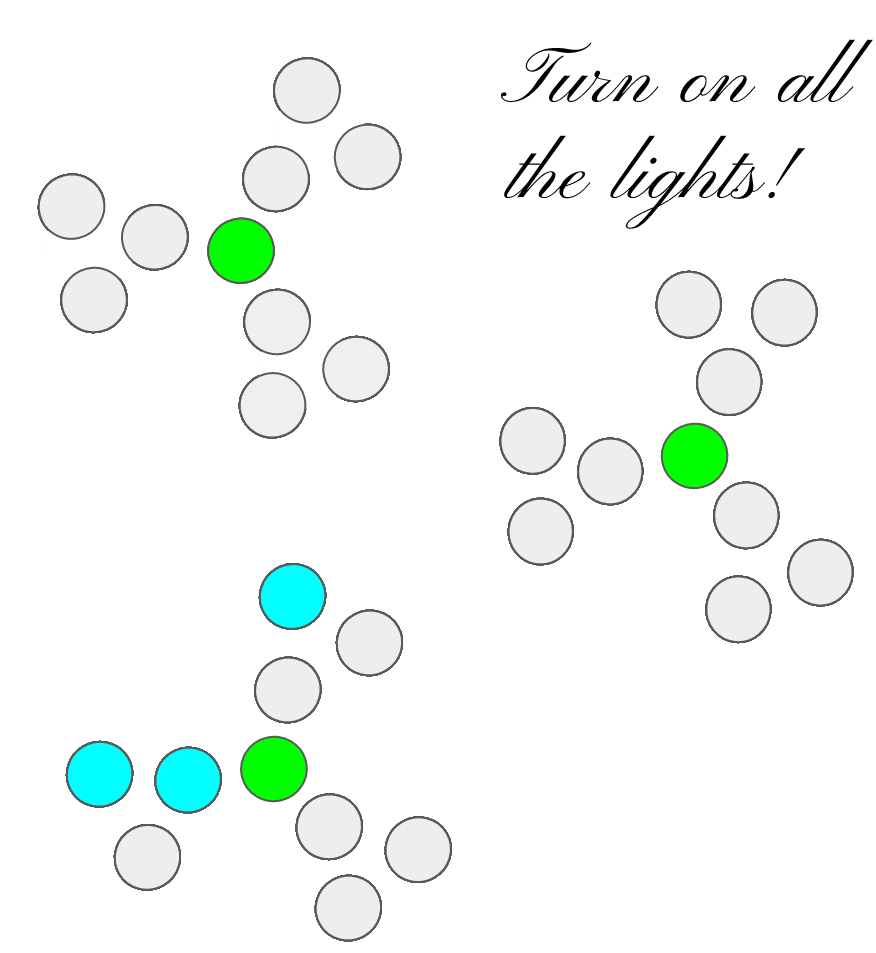
\includegraphics[width=0.5\linewidth]{NIPSfigures/Task.png}
  \caption{Example illustration of the task. At the current state, three level-0 lights (blue) are on, all level-1 lights are off (invisible) and all three level-2 lights are on, meaning that they will be replaced with a single level-3 light in this turn. The agent's goal is to turn on "all the lights".}
  \label{TaskFigure}
\end{figure}


\subsection{Reinforcement learning agents}

We created and compared several different reinforcement learning agents in their performance on this task. Agents were either driven by reward or novelty (or a combination of both); and agents either chose among basic actions only (flat) or created abstract options, from which they could select in addition to the basic actions (hierarchical). Although only a subsection of agents was hierarchical, we will refer to all actions and options as options from now on.

All agents used tabular methods for option-value learning and selected options based on values in an epsilon-greedy fashion, $P(a_{max}) = 1 - \epsilon$, whereby $a_{max}$ represents the action or group of actions with the currently highest state-action value and $\epsilon$ is the small probability of selecting an option with a value that is not the largest available. $P(a \neq a_{max}) = \epsilon$, whereby $a$ represents the option or group of options with non-maximum values. Probabilities were divided equally in the case of multiple optimal or non-optimal options. 


\subsubsection{Flat agents}

Sisyphus, the flat, reward-driven agent learned a separate option-value for each of its two options (turn-off and turn-off) for each available light. The Sisyphus agent perceived an outcome as rewarding when the number of level-0 on-lights increased, $r_t = n_t^{on} - n_{t-1}^{on}$, whereby $n^{on}$ represents the number of lights that are currently on. The agent updated its option values using classic Rescorla-Wagner updates, $v(a) = v(a) + \alpha (r - v(a))$, with learning rate $\alpha$.

The flat, novelty-driven agent was similar to Sisyphus expect that it updated option-values based on novelty $n$ rather than reward, $v(a) = v(a) + \alpha (n - v(a))$. Novelty was calculated as $n = \frac{1}{count}$, where $count$ keeps track of the number of times each event, i.e., lights turning on and off, has occurred. 

The combined reward-novelty agent used a linear combination of the novelty and reward signals to update option-values, $v(a) = v(a) + \alpha (r + n - v(a))$. 


\subsubsection{Hierarchical agents}

Socrates, the hierarchical, novelty-driven agent, used novelty to guide option creation and the calculation of option-values. Novelty was different in the hierarchical agent compared to the flat agents because it also encompassed higher-level lights. (To facilitate comparison, we also constructed a flat agent that perceived higher-level novelty, with similar results.)

The Socrates agent kept a count for each event (level-0 lights and higher-level lights) to determine its novelty, similar to the flat novelty-seeking agent. Option values were updated based on novelty, like above, with the addition of temporal discounting to account for the delay induced by the execution of an option. The Socrates agent also created a new option each time it perceived a novel event, i.e., $n \geq 1$. An option's initiation set consisted of the whole state space, i.e., each option could be initiated at all times. An option terminated when the agent was successful in reinstating the event for which the option had been created, i.e., when the same higher-level light turned on again. Options also terminated with a small percentage at each time step, such that unsuccessful options did not continue forever. 

Once created, options could be reused in higher-level options. This means that options can be very efficient, pointing to just $n_{tuple}$ options (or actions) at the level directly below.

Within-option policies were learned in the following way: Each option was associated with a separate option-value table. Values in this table reflected the expectation of reaching the option goal upon selecting each option. When an option was created, the values of all available options were initialized at 0, expect for the option executed immediately prior to the formation of the option, which was set to 1. Subsequently, whenever an option's goal was reached, i.e., its corresponding higher-level light turned on, the value of the option executed immediately before was set to 1. In this way, option policies were updated whether or not an option was currently in charge of option selection. 

Hierarchical agents selected among options. When a 1-step option (basic action) was selected, it was executed and its value updated according the equations given above. When a multi-step option was selected, within-option values were used to guide action selection until the option terminated. If the option terminated successfully (sub-goal reached), it's value was updated according to the novelty of the event, plus the novelty accrued during option execution. If the option terminated unsuccessfully, it's value was updated according to only novelty accrued during execution. 

The hierarchical, reward-seeking agent was similar to the Socrates agent except that it updated values according to reward, rather than novelty.


\section{Results}

\subsection{Flat agents}

\begin{figure}[h]
  \centering
  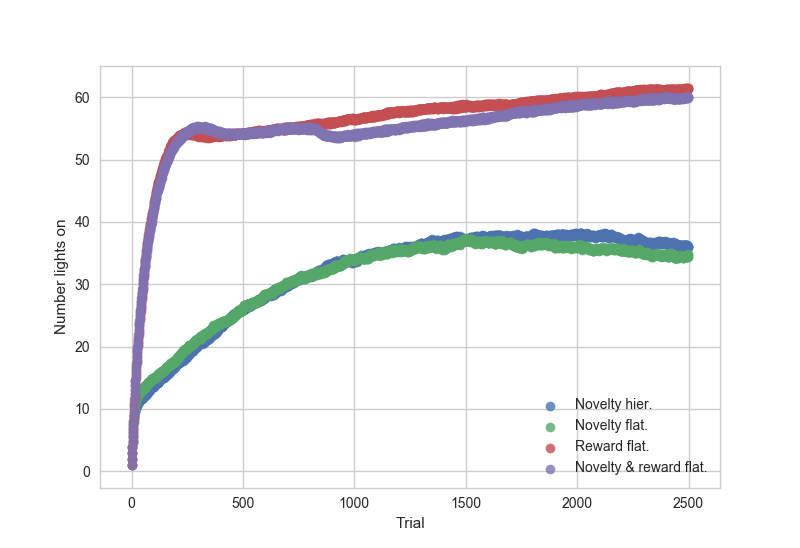
\includegraphics[width=\linewidth]{NIPSfigures/NLights.png}
  \caption{Comparison of the four flat agents in terms of number of lights turned on. The agents played games with 81 lights, which were organized into groups of 3. Shown are the means of 50 agents of each category. All agents had a learning rate of 75\% and epsilon of 5\%. Legend: "Novelty hier." refers to the flat agent that perceives basic- and higher-level lights; "Novelty flat": flat agent, flat novelty; "Reward flat": flat agent, driven by rewards; "Novelty \& reward flat": flat agent, driven by the sum of novelty and reward.}
  \label{ResultsFlatFigure}
\end{figure}

As expected, neither of the flat agents were able to win a game of 81 lights with 3 lights per group, i.e., the agents did not succeed in turning on all 81 lights within a reasonable time frame (see Figure \ref{ResultsFlatFigure}). Reward-driven agents surpassed novelty-driven agents. 

Reward-driven agents quickly increased the number of turned-on lights in this game. These agent learned that the turn-on action resulted in rewards for most of the lights, whereas the turn-off action resulted in punishment. The agents therefore tended to repeat on-actions when they were available, but avoided off-actions, thereby increasing the overall number of on-lights. Within 200 trials, the reward-agents had turned on an average of 54 lights, exactly two-thirds of the 81 available lights. The number of turned-on lights then remained relatively stable for more than 500 trials. The reason for this is that the agents had received negative rewards for one out of three turn-on action (whenever a higher-level light turned on and three level-0 lights turned off), resulting in a large negative reward of -2 for one specific turn-on action. The agents therefore avoided these turn-on actions and would even prefer turning off lights (expected reward of -1) to turning on these lights again (expected reward of -2). The reason that the number of lights increased slowly thereafter is the noise in agents' epsilon-greedy selection rule. 

Flat novelty-driven agents increased the number of turned-on lights much more slowly than reward-agents. The novelty-driven agents explored actions randomly, being rewarded with equal novelty for each action irrespective of whether it turns lights on or off. Flat novelty-agents "wanted" to repeat newly-discovered actions as soon as possible, having assigned high novelty values to it after their first discovery. But the environment does not allow agents to turn on lights that are already on, such that they need to wait until a group of lights turns off in junction, such that it can turn them all on again, or until it discovers the off-action that corresponds to a previously-performed on-action. At this point, both on- and off-actions have high values and agents perform them in turn for many trials, continuously reducing both actions' novelty. With the next non-greedy action selection, the agent has a new chance of discovering an action that is the counterpart of an already-discovered action; if it is found, the agent will execute these two actions in turn, and so on, until eventually, all actions have been discovered. Resembling a random process, the agent's behavior pushed the number of turned-on lights slowly but consistently toward its expected value, the mean of 40.5 lights. There are two reasons this number was not reached: First, the environment turned groups of lights off according to the rules, reducing the number of on-lights; and second, the agent never managed to explore all actions because it spent too much time playing with pairs of corresponding actions. 

The agent that combines novelty and reward resembled the pure reward agent. 

Taken together, both kinds of flat agent showed behaviors that were promising for learning in this task, but not sufficient. The reward-agent misattributed a group of lights turning off to one particular action, and therefore stopped exploring these actions further. The novelty-agent was not motivated to turn on lights, rather than turning the off, and therefore just "played" with the lights, reducing novelty over time. Both agents also lacked the capability of understanding the underlying mechanism of the game, being limited to learning about single actions rather than more complex structures. 


\subsection{Hierarchical agents}

We expect that hierarchical agents will remedy the shortcomings of the flat agents. In specific, we expect that agents that are purely driven by novelty will succeed in this task, even without a notion reward. The reason for this is that in hierarchical agents, novel events will trigger the creation of an option with the sub-goal of achieving the same event again. New options will be initialized with high values, corresponding to the initial high novelty of the event. Agents will therefore be motivated to (1) learn how to achieve the same outcome again and (2) to achieve the same outcome again. By repeating to turn on higher-level lights, agents will unlock higher levels, experience more novelty, create more options (which can be based on options for lower levels), unlock more levels, and so on, until all lights are finally turned on. We therefore expect that hierarchical, novelty-driven agents can win this game, even though they do not possess a notion of reward.


\subsection{Motivation}

We lastly compared the values that each kind of agent assigned to the different actions. As expected, the reward agent learned to assign positive values to on-actions and negative values to off-actions. Average values for on-actions decreased suddenly after 150 trials as re-trying actions of initial high values led to the unexpected turning off of lights. Values increased slowly thereafter, as high-level events became more and more sparse. The values of off-actions decreased steadily as the agent learned that these always lead to negative rewards.

Surprisingly, the novelty agent assigned larger average values to on- than off-actions. The reason for this is that more on- than off-actions show values of 0.75 at the end of the game, revealing that they were discovered once, but that the corresponding off-action was never discovered. Most other actions had either very small values (because they were part of a "game", in which the agent turned a single light on and off repeatedly), or the initial value of 0 (because they were never tried). The reason that more on- than off-action had values of 0.75 is that the mechanics of the game itself switching off some lights, leaving the agent with more options among on- than off-actions, such that many on-action were explored whose off-counterpart remained unexplored. The average value of on-actions first increased steadily, as more and more actions were discovered. After a turning point around 1200 trials, the average value slowly decreased because all actions lost their novelty as the agent circled through them in the search of the most novel one.

Importantly, the average values of all lights were strictly positive for the novelty-agent, but negative for the reward-agent. In other words, the novelty agent showed what would be called approach behavior in psychology, whereas the reward-agent showed avoidance behavior. 

\begin{figure}[h]
  \centering
  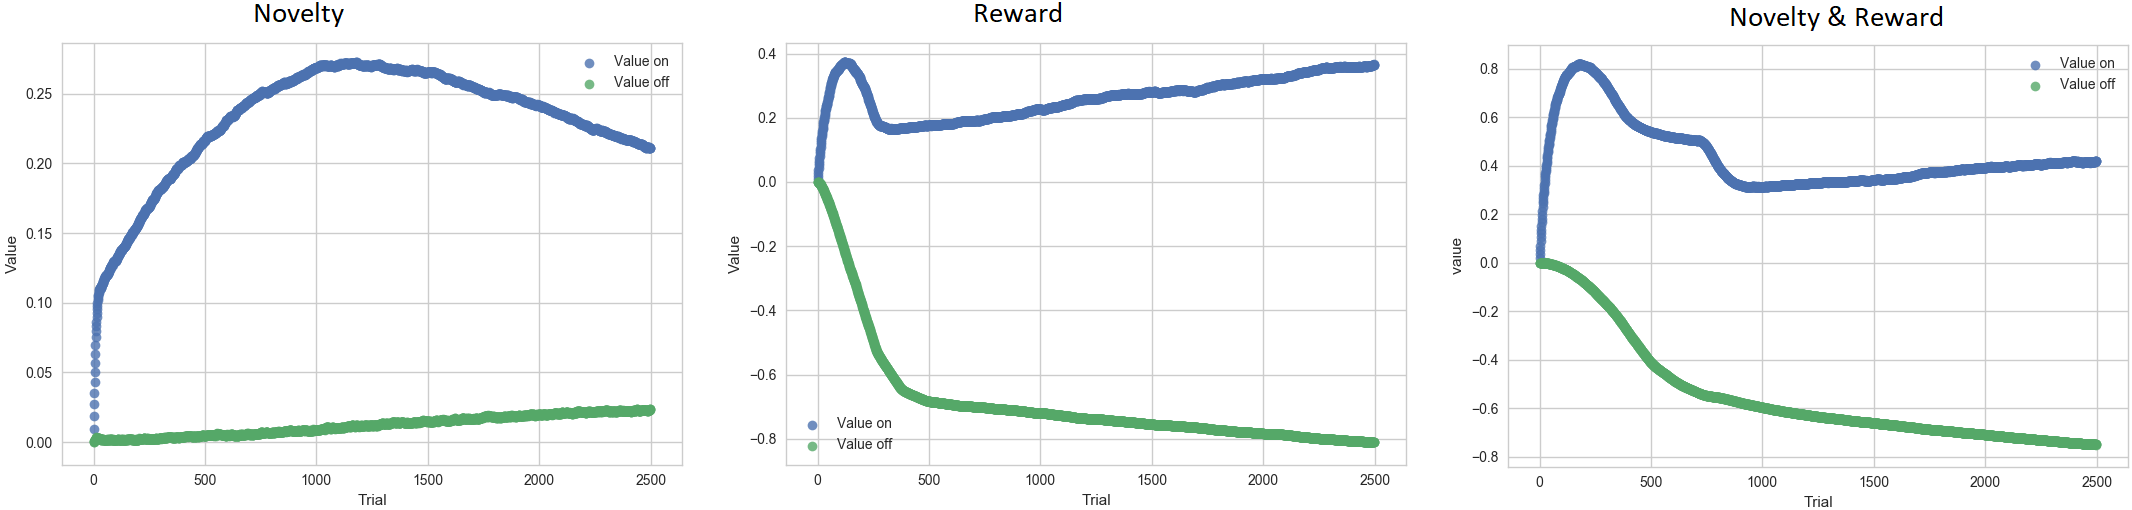
\includegraphics[width=\linewidth]{NIPSfigures/VFlat.png}
  \label{ResultsFlat}
  \caption{Comparison of the flat agents in terms of action-values for the on- and off-actions. Same games as before.}
\end{figure}

For the hierarchical novelty-driven agent, values will be overall positive like for the flat novelty-driven agent. We expect that this agent will be able to avoid the "play"-circle of turning the same light on and off repeatedly through the use options. The increased use of options should lead to broader exploration.


\section{Conclustion}

We have introduced a novel task paradigm that is suited to pit exploratory and exploitatory behavior against each other, shedding some light on novel debates arising between classical reinforcement learning based on reward, and novel approaches that have highlighted the power of novelty alone as a driving force of learning. We have shown that reward alone is better suited to motivate flat agents to perform well in a task, but that reward-motivated flat agents do not reach the final goal of the task. (None of the 200 simulated flat agents actually won the game, i.e., managed to turn on all the lights, within 2500 trials.)

We have also highlighted differences in the behavior of reward- versus novelty-driven agents. Most notably, reward-driven agents were motivated to avoid expected negative consequences, whereas novelty-driven agents were motivated to seek expected positive outcomes. This difference might have implications for other tasks and might even help elucidate psychological phenomena such as learned helplessness (Sisyphus agent) and optimism (Novelty-seeking agent). 

We have proposed the abstract framework of a game-like task, but think that the proposed algorithm of the Socrates agent might be meaningful for a wide range of psychological phenomena. The idea of combining novelty-seeking with hierarchical learning might be able to shed some light on areas as different as motor learning, language learning, and concept formation. In each of these, behavior starts from simple "level-0" actions, e.g., phonemes in the realm of language or simplest body movements in the realm of motor learning. In both cases, learners, usually infants, are motivated to explore the outcomes of their actions, thereby reducing uncertainty over time. At the same time, the formation of hierarchical actions. 

Several extensions are possible to the current framework. It would be worth exploring how results would differ if the same basic underlay all higher-level events. This scenario might be closer to many real-world learning situations, such as motor and language learning. Another place for exploration would be order. In the given example, order was irrelevant for the creation of higher-level events, but order is indeed crucial in many situations. It would also be worth exploring what would happen if there were only on-, but no off-actions, which would come closer the notion of actions in the real world, in which "un-actions" do not exist. 

This paradigm could also be tested in human, such that learning could be characterized in terms of goal and structure.

Taken together, by creating the hierarchical novelty-seeking Socrates agent, we hope to show that learning of meaningful behavior can be driven by learning itself, rather than external rewards. In this framework, the learner produces the crucial learning signals itself, by selecting actions that reduce novelty and surprise over time. In other words, this learner balances the search for novelty with reducing prediction errors. It explores the environment in a systematic way, forms "hypotheses" and conducts "experiments", in order to learn more. 

\section*{References}

\printbibliography

\end{document}